\section{Постановка задачи}

\glsxtrnewsymbol[description={пространственная координата вдоль сосуда, [м]}]{x}{\ensuremath{x}}
\glsxtrnewsymbol[description={время, [с]}]{t}{\ensuremath{t}}
\glsxtrnewsymbol[description={площадь поперечного сечения сосуда в фиксированном сечении, [м\textsuperscript{2}]}]{a}{\ensuremath{a}}
\glsxtrnewsymbol[description={$=\sqrt{a/\pi}$, радиус сосуда, [м]}]{R}{\ensuremath{R}}
\glsxtrnewsymbol[description={средняя по поперечному сечению сосуда скорость жидкости, [м/с]}]{u}{\ensuremath{u}}
\glsxtrnewsymbol[description={среднее по поперечному сечению сосуда давление, [Па]}]{p}{\ensuremath{p}}
\glsxtrnewsymbol[description={плотность жидкости, [кг/м\textsuperscript{3}]}]{rho}{\ensuremath{\rho}}
\glsxtrnewsymbol[description={динамическая вязкость жидкость, [Па$\cdot$c]}]{mu}{\ensuremath{\mu}}
\glsxtrnewsymbol[description={нормированная на общий радиус $R$ радиальная координата сосуда, [1]}]{r_prime}{\ensuremath{r'}}
\glsxtrnewsymbol[description={нормированный профиль скорости, [1]}]{U}{\ensuremath{U}}
\glsxtrnewsymbol[description={параметр, описывающий радиально-симметричный профиль скорости, [1]}]{zeta}{\ensuremath{\zeta}}
\glsxtrnewsymbol[description={параметр, описывающий эластичные свойства материала стенки сосуда, [кг/с\textsuperscript{2}]}]{beta}{\ensuremath{\beta}}
\glsxtrnewsymbol[description={модуль упругости стенки сосуда, [Па]}]{E}{\ensuremath{E}}
\glsxtrnewsymbol[description={толщина стенки сосуда, [м]}]{h}{\ensuremath{h}}
\glsxtrnewsymbol[description={площадь поперечного сечения сосуда сосуда при отсутствии внешнего воздействия, [м\textsuperscript{2}]}]{A}{\ensuremath{A}}
\glsxtrnewsymbol[description={объёмный расход жидкости, [м\textsuperscript{3}/с]}]{q}{\ensuremath{q}}

\subsection{Определяющая система уравнений}
Для выводы определяющей системы уравнений будем следовать подходу~\cite{Hughes1973}
с некоторыми упрощениями.

\subsubsection{Осреднение по сечению сосуда}

\begin{figure}[h]
    \centering
    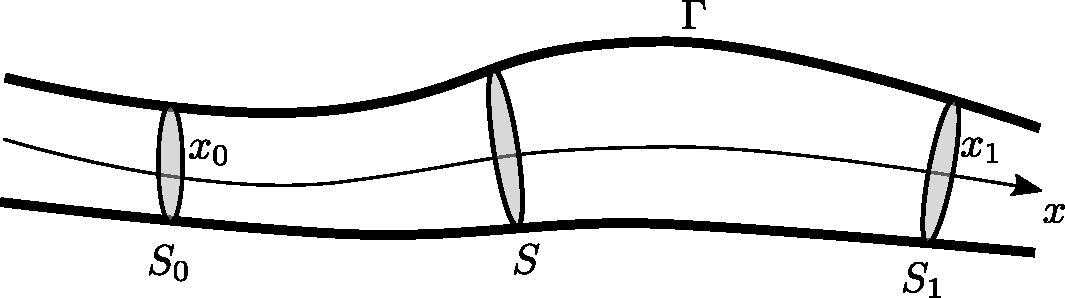
\includegraphics[width=0.6\linewidth]{def.pdf}
    \caption{Элементарный объём $V$}
    \label{fig:elementary_volume}
\end{figure}

Будем рассматривать течение в сосуде с продольной координатой \gls{x}.
Определим элементарный объём $V$ как отрезок сосуда при $x\in[x_0, x_1]$ (см. рис.~\ref{fig:elementary_volume}).
Границей этого объема будут входное и выходное сечения $S_0$, $S_1$ и
боковая граница $\Gamma$: $\partial V = S_0 \cup S_1 \cup \Gamma$.

Пусть величина $g$ переносится в этом элементарном объёме несжимаемой
жидкостью со скоростью $\vec u$:
\begin{equation}
\label{eq:divu}
\nabla\cdot \vec u = 0.
\end{equation}
Тогда распишем изменения по времени \gls{t}  интеграла от этой величины $g$ согласно теореме Рейнольдса:
\begin{equation}
\label{eq:reynolds-transport}
\frac{d}{dt}\int\limits_{V}g\,d\vec x = 
\int\limits_{V}\dfr{g}{t}\,d\vec x + \int\limits_{\partial V} g v_n \,d s
\end{equation}
Здесь $v_n$ -- нормальная скорость объема $V$.
Будем считать, что объём не совершает продольного движения. То есть
\begin{equation}
\label{eq:zero_vn}
\left.v_n\right|_{S_0, S_1} = 0.
\end{equation}
Определим среднее по сечению значение как
\begin{equation}
\label{eq:average_g}
\bar g = \frac{1}{|S|}\int\limits_S g \, ds.
\end{equation}
Тогда, с учётом того, что координаты $x_0$, $x_1$ не зависят
от времени (как следствие из \cref{eq:zero_vn}), левая часть \cref{eq:reynolds-transport} может быть представлена
в виде
\begin{equation}
\label{eq:left_in_reynolds_transport}
\frac{d}{dt}\int\limits_{V}g\,d\vec x = 
\int\limits_{x_0}^{x_1} \dfr{|S| \bar g}{t} \, dx.
\end{equation}

Далее рассмотрим второе слагаемое в правой части \cref{eq:reynolds-transport}.
Обозначим за $w_n$ -- скорость объема относительно $u_n$ -- скорости жидкости:
\begin{equation}
\label{eq:wn_vn_un}
w_n = v_n - u_n.
\end{equation}
\begin{equation}
\label{eq:second_in_reynolds_transport}
\int\limits_{\partial V} v_n g \, ds = 
\int\limits_{\partial V} w_n g \, ds +
\int\limits_{\partial V} u_n g \, ds.
\end{equation}
Для первого слагаемого в правой части \cref{eq:second_in_reynolds_transport} справедливо

\begin{align*}
\int\limits_{\partial V} w_n g \, ds
	& = \int\limits_{\Gamma} w_n g \, ds
	  + \int\limits_{S_0} w_n g \, ds
	  + \int\limits_{S_1} w_n g \, ds = \dots \\
\intertext{расписывая $w_n$ по \cref{eq:wn_vn_un} с учётом \cref{eq:zero_vn}}
	& = \int\limits_{\Gamma} w_n g \, ds
	  - \int\limits_{S_0} u_n g \, ds
	  - \int\limits_{S_1} u_n g \, ds = \dots \\
\intertext{подставляя определение \cref{eq:average_g} для произведения $u_n g$}
	& = \int\limits_{\Gamma} w_n g \, ds
	  - \left(|S|\overline{u_n g}\right)_{x_0}
	  - \left(|S|\overline{u_n g}\right)_{x_1} = \dots \\
\intertext{заменим нормальную скорость $u_n$ скоростью $u_x$ по направлению координаты $x$ с учётом направления внешней нормали в сечениях $x_0$, $x_1$}
	& = \int\limits_{\Gamma} w_n g \, ds
	  + \left(|S|\overline{u_x g}\right)_{x_0}
	  - \left(|S|\overline{u_x g}\right)_{x_1} = \dots\\
\intertext{применяя формулу интегрирования по частям}
	& = \int\limits_{\Gamma} w_n g \, ds
	  - \int\limits_{x_0}^{x_1} \dfr{|S| \overline{u_x g} }{x} \, dx.
\end{align*}

Второе слагаемое в правой части \cref{eq:second_in_reynolds_transport} распишем по формуле Гаусса-Остроградского
с учётом условия неразрывности \cref{eq:divu}:
\begin{equation}
\nonumber
\int\limits_{\partial V} u_n g \, ds =
\int\limits_{V} \vec u \cdot \nabla g \, d\vec x
\end{equation}

Собирая равенство \cref{eq:reynolds-transport} с учётом полученных соотношений получим
\begin{equation}
\nonumber
\int\limits_{x_0}^{x_1} \left( \dfr{|S| \bar g}{t} + \dfr{|S| \overline{u_x g} }{x}\right) \, dx =
\int\limits_V \left(\dfr{g}{t} + \vec u \cdot \nabla g \right)\, d\vec x
+ \int\limits_{\Gamma} w_n g \, ds
\end{equation}
Далее, пользуясь произвольностью выбора продольной координаты снимем интегрирование по $x$:
\begin{equation}
\label{eq:common_s_average}
\dfr{|S| \bar g}{t} + \dfr{|S| \overline{u_x g} }{x} =
\int\limits_{S(x)} \left(\dfr{g}{t} + \vec u \cdot \nabla g \right)\, ds
+ \oint\limits_{L(x)} w_n g \, dl.
\end{equation}
Здесь $L$ -- сечение поверхности $\Gamma$ по фиксированной продольной координате $x$.

\subsubsection{Сохранение массы}
Для получения закона сохранения массы рассмотрим общее
соотношение \cref{eq:common_s_average} при $g = 1$:
\begin{equation}
\nonumber
\dfr{|S|}{t} + \dfr{|S| \overline{u_x} }{x} =
\oint\limits_{L(x)} w_n \, dl.
\end{equation}
Интеграл в правой части -- есть расход жидкости через 
боковые стенки сосуда. В настоящей работе мы ограничимся
случаем непроницаемых стенок сосуда:
\begin{equation}
\nonumber
\left.w_n \right|_\Gamma = 0,
\end{equation}
Тогда этот интеграл будет равен нулю.
Для величин в левой части введём обозначения:
$\gls{a} = |S|$ -- площадь поперечного сечения сосуда, равная $a = \pi \gls{R}^2$.
$\gls{u} = \bar u_x$ -- средняя по сечению продольная скорость жидкости.
Тогда закон сохранения масс примет вид
\begin{equation}
\label{eq:mass_conservation}
\dfr{a}{t} + \dfr{u a}{x} =0
\end{equation}

\subsubsection{Сохранение количества движения}
Рассмотрим уравнения \cref{eq:common_s_average}
при $g = u_x$. С учётом введённых обозначений получим
\begin{equation}
\label{eq:momentum_first}
\dfr{a u}{t} + \dfr{a \bar u_x^2 }{x} =
\int\limits_{S(x)} \left(\dfr{u_x}{t} + \vec u \cdot \nabla u_x \right)\, ds
+ \oint\limits_{L(x)} w_n u_x \, dl.
\end{equation}

Для последующих выкладок сделаем допущение, что форма профиля скорости вдоль всей длины сосуда постоянна (не зависит от координаты $x$)
и радиально-симметрична (зависит только от нормированной радиальной координаты $\gls{r_prime} = r/R$).
То есть $u_x$ представима в виде
\begin{equation}
\label{eq:ux_simplification}
u_x(x, s) = u(x) U(r'),
\end{equation}
где \gls{U} -- нормированный профиль скорости.

Правую часть распишем с использованием ранее выведенного закона сохранения масс \cref{eq:mass_conservation}:
\begin{align}
\dfr{a u}{t} + \dfr{a \bar u_x^2 }{x}
   & = a\dfr{u}{t} - u\dfr{au}{x} + \dfr{a \bar u_x^2 }{x} = \dots\nonumber\\
\intertext{добавим и вычтем слагаемое $\dsfr{au^2}{x}$}
   & = a\dfr{u}{t} - u\dfr{au}{x} + \dfr{au^2}{x} + \dfr{a (\bar u_x^2 - u^2)}{x} = \dots\nonumber\\
\intertext{разложим третье слагаемое и проведём сокращения}
   & = a\dfr{u}{t} + au\dfr{u}{x} + \dfr{a (\bar u_x^2 - u^2)}{x} = \dots\nonumber \\
\intertext{воспользуемся упрощением \cref{eq:ux_simplification}}
   & = a\dfr{u}{t} + au\dfr{u}{x} + (\bar U^2 - 1)\dfr{a u^2}{x}\label{eq:momentum_first_left}.
\end{align}

Упрощение первого интеграла в правой части будем проводить на
основе общего уравнения движения для вязкой несжимаемой жидкости, записанного в проекции на ось $x$:
\begin{equation}
\label{eq:ns_ux}
\dfr{u_x}{t} + \vec u \cdot \nabla u_x = -\frac{1}{\rho} \dfr{p}{x} + \frac{\mu}{\rho}\nabla^2 u_x,
\end{equation}
где \gls{p} -- давление, \gls{rho} -- плотность и \gls{mu} -- вязкость жидкости.
Будем считать,
что продольные изменения скорости намного меньше, чем поперечные. Это справедливо, если справедливы условия
прилипания к боковым стенкам канала. Тогда можно записать
\begin{equation}
\nonumber
\nabla^2 u_x = \nabla^2_S u_x + \dfrq{u_x}{x} \approx \nabla^2_S u_x,
\end{equation}
за $\nabla^2_S$ обозначен двумерный оператор Лапласа, действующий в плоскости $S$.
Подставим это приближение в выражение \cref{eq:ns_ux} 
и проинтегрируем по плоскости $S$:
\begin{align}
\int\limits_S\left(\dfr{u_x}{t} + \vec u \cdot \nabla u_x\right)\, ds
	& = -\frac{1}{\rho} \int\limits_S\dfr{p}{x}\, ds + \frac{\mu}{\rho}\int\limits_S\nabla^2_S u_x \, ds = \dots\nonumber\\
\intertext{будем считать, что давление слабо меняется поперёк канала: $p(x, s)\approx\bar p(x)$}
	& = -\frac{1}{\rho} |S|\dfr{p}{x} + \frac{\mu}{\rho}\int\limits_S\nabla^2_S u_x \, ds = \dots\nonumber\\
\intertext{и раскроем второй интеграл с помощью интегрирования по частям}
	& = -\frac{1}{\rho} |S|\dfr{p}{x} + \frac{\mu}{\rho}\oint\limits_L \dfr{u_x}{n_l} \, dl = \dots\nonumber\\
\intertext{в радиально-симметричном упрощении, при котором $n_l = r$}
	& = -\frac{1}{\rho} |S|\dfr{p}{x} + \left.\frac{2\pi\mu R}{\rho}\dfr{u_x}{r}\right|_{r=R(x)} = \dots\nonumber\\
\intertext{воспользуемся упрощением \cref{eq:ux_simplification} для вычисления последней производной}
	& = -\frac{1}{\rho} |S|\dfr{p}{x} + \left.\frac{2\pi \mu}{\rho} u \dfr{U}{r'}\right|_{r'=1} \label{eq:momentum_first_right}
\end{align}

Запишем уравнение \cref{eq:momentum_first} с учётом \cref{eq:momentum_first_left,eq:momentum_first_right}:
\begin{equation}
\label{eq:momentum_second}
\dfr{u}{t} + u\dfr{u}{x} + \frac{\bar U^2 - 1}{a}\dfr{a u^2}{x} =
	-\frac{1}{\rho} \dfr{p}{x} + \left.\frac{2\pi\mu}{\rho}\frac{u}{a}\dfr{U}{r'}\right|_{r'=1}.
\end{equation}

Для проведения дальнейших упрощений необходимо допущение о форме профиля $u_x(r, x)$.
В простейшем случае можно считать его постоянным: $U=1$. Тогда вследствие $u_x(r, x) = u(x)$
выражение \cref{eq:momentum_second} преобразуется к виду
\begin{equation}
\label{eq:momentum_conservation_inviscid}
\dfr{u}{t} + u\dfr{u}{x} = -\frac{1}{\rho} \dfr{p}{x}.
\end{equation}
Таким образом, мы получили уравнение движения при полном пренебрежении
силами вязкого трения о стенки сосуда.

\subsubsection{Учёт вязкого трения}
Рассмотрим радиально-симметричный случай, при котором профиль задаётся соотношением
Рассмотрим радиальный профиль скорости \gls{U}, который задаётся соотношением (см.~\cite{Hughes1973,Smith2001})
\begin{equation}
U_0(r') = \frac{\zeta+2}{\zeta} \left(1 - \left(r'\right)^{\zeta}\right),
\end{equation}
через параметр \gls{zeta}. Случай $\zeta=2$ соответствует установившемуся профилю Пуазейля.
Более высокие значение $\zeta$ отражают неустановившийся характер течения.
Профили для некоторых $\zeta$ представлены на рис.~\ref{fig:U}.


\begin{figure}[h]
    \centering
    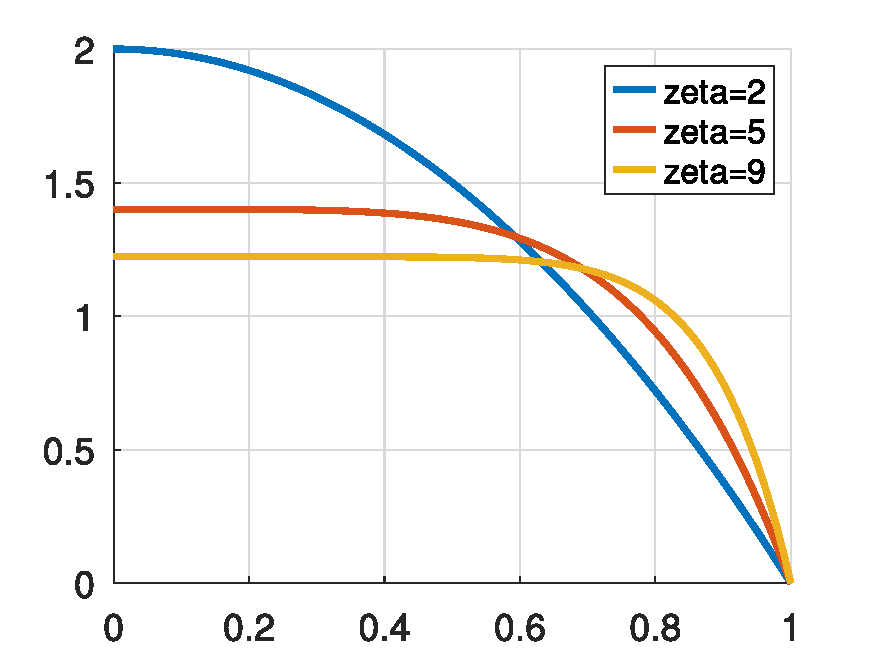
\includegraphics[width=0.4\linewidth]{U.pdf}
    \caption{Нормированный профиль скорости в зависимости от $\zeta$}
    \label{fig:U}
\end{figure}

Выражения из \cref{eq:momentum_second}, содержащие нормированную скорость, будут равны:
\begin{align*}
\left.\dfr{U}{r'}\right|_{r'=1} &= - (\zeta+2),\\
\bar U &= 1,
\end{align*}
тогда само уравнение сохранения количества движения примет вид
\begin{equation}
\label{eq:momentum_conservation_viscous}
\dfr{u}{t} + u\dfr{u}{x} =
	-\frac{1}{\rho} \dfr{p}{x} - \frac{2\pi\mu(\zeta+2)}{\rho}\frac{u}{a}.
\end{equation}

\subsubsection{Замыкающее соотношение для давления}
Постановка задачи включает в себя два соотношения \cref{eq:mass_conservation,eq:momentum_conservation_viscous}
для трёх неизвестных $u$, $a$, $p$. Таким образом, необходимо ещё одно,
замыкающее соотношение.
Обычно таким соотношением служит зависимость давления от площади поперечного сечения $p(a)$.
Следуя~\cite{Formaggia2003} запишем это соотношение в приближении равновесного состояния (давление мгновенно подстраивается под изменение площади сечения сосуда)
при условии нулевого внешнего давления.
\begin{equation}
\nonumber
p(a) = \frac{\beta}{A} \left(\sqrt{a} - \sqrt A\right).
\end{equation}
Здесь \gls{A} -- нейтральный радиус сосуда,
а коэффициент \gls{beta} вычисляется в приближении тонкой, несжимаемой, однородной, изотропной, эластичной мембраны с толщиной \gls{h} и 
модулем упругости \gls{E}:
\begin{equation}
\nonumber
\beta = \frac{4}{3}\sqrt{\pi}E h.
\end{equation}

\subsection{Характеристический анализ}
TODO

\subsection{Граничные условия и условия на разрывах}
TODO

\subsubsection{Выходное условие}
TODO

\subsubsection{Входное условие}
Во входном сечении сетки сосудов обычно задают либо входной профиль давления $p_{in}(t)$
либо общий расход $\gls{q}_{in}(t)$. На выходе -- неотражающие выходные условия.

\subsubsection{Условие в точке разрыва свойств сосуда}
TODO

\subsubsection{Условие в точке разветвления}
TODO
